In this section, we will first elaborate on the benchmarking deep neural networks that we choose, then we run them in 3 kinds of GPU frequencies to obtain the power, performance, and temperature profiles. These profiles act as the baseline for the study of the CPU-GPU execution scenario.

\paragraph{Benchmarks}

We try to pick small, medium, and large deep neural networks in terms of the depth of the network. Specifically, we pick 3 neural networks from those that are used to tackle image classification task of the ImageNet dataset. We summarize the benchmark we choose in Table.~\ref{table:1}. We measure the memory overhead by using \textit{tegrastat} provided by NVIDIA while inferencing the image.

Notice that there is only 4GB of RAM available on TX1, which is shared between CPU and GPU, with 1GB reserved by the operating system (Ubuntu). Hence, in the case of ResNet-152, it almost consumes all the available memory of the system that might leave barely nothing for the CPU. On the other hand, the shallowest neural network we have is AlexNet, and it still consumes a large amount of memory, i.e. 720 MB.


\begin{table}[h]
    \begin{center}
        \begin{tabular}{ | c | c | c | c | }
        \hline
        & Memory (MB) & \# Layers & Top-1 Acc. \\ \hline
        AlexNet{\cite{krizhevsky2012imagenet}} & 720 & 7 & 57.2\% \\ \hline
        GoogLeNet{\cite{szegedy2015going}} & 820 & 22 & 68.7\%  \\ \hline
        ResNet-152{\cite{he2016deep}} & 2224 & 152 & 77.0\% \\
        \hline
        \end{tabular}
    \end{center}
    \caption{The descriptions of the deep neural networks we choose, including the memory overhead during inference (single image), number of layers, and the reported top-1 accuracy on ImageNet.}\label{table:1}
\end{table}

We choose 3 kinds of GPU voltage/frequency pairs, i.e. the smallest (0.82 V, 76.8 Mhz), the medium (0.85 V, 537.6 Mhz), and the largest (1.1 V, 998.4 Mhz), from the 13 available voltage and frequency pairs on NVIDIA Tegra X1 to further investigate the power, latency, and temperature profiles of the aforementioned benchmarks.

\paragraph{Profiling}

We sweep through 3 different voltage and frequency pairs for each of the benchmark that we study and collect the temperature of both CPU and GPU, the power consumption of the GPU, and the latency of the tasks.

\begin{figure}[h]
    \centering
    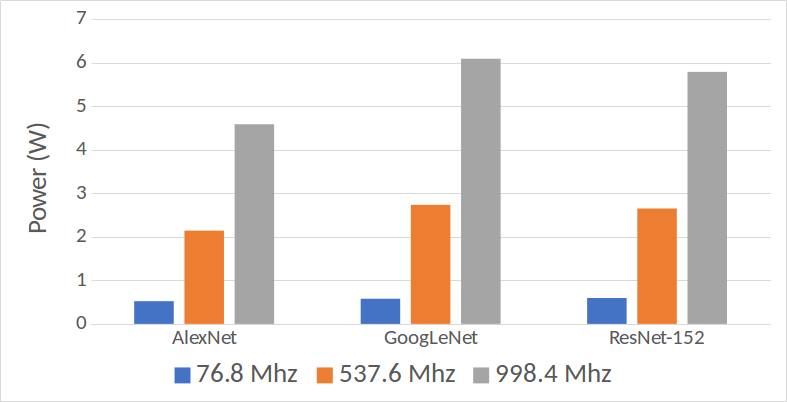
\includegraphics[width=0.5\textwidth]{power_profile.png}
    \caption{The power profile when running DNN benchmarks under different GPU voltage/frequency pairs.}\label{fig:1}
\end{figure}

\begin{figure}[h]
    \centering
    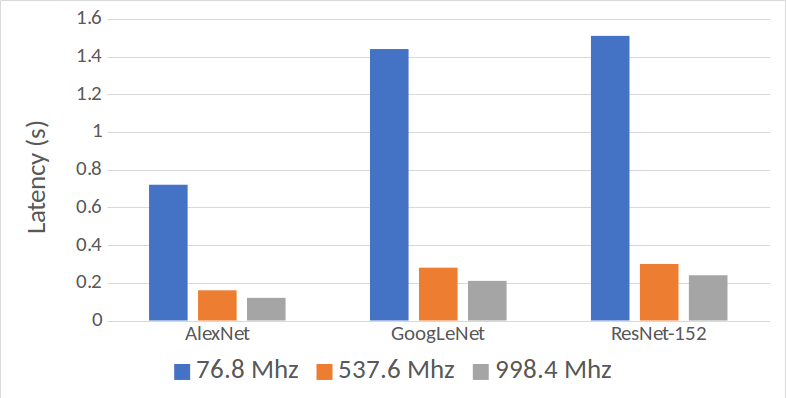
\includegraphics[width=0.5\textwidth]{latency_profile.png}
    \caption{The latency profile when running DNN benchmarks under different GPU voltage/frequency pairs.}\label{fig:2}
\end{figure}

Fig.~\ref{fig:1} and Fig.~\ref{fig:2} show both the power and latency profile of the aforementioned DNN benchmarks running under different GPU voltage/frequency pairs. As expected, the power consumption is higher when the GPU voltage and frequency are higher. Also, the deeper the neural network the higher the latency. Interestingly, the power consumption of GoogLeNet is higher than ResNet-152 at each voltage and frequency pair, which implies that the utilization of the GPU when runnnig GoogLeNet is higher than ResNet-152. On the other hand, the three benchmarks share similar temperature profiles, i.e. around 40C on average, which is far from the throttling temperature of the GPU on TX1, i.e. 89.5C.

To further compare and analyze the characteristics of these benchmarks, we normalize the latency, power consumption, and accuracy to AlexNet as shown in Fig.~\ref{fig:3}. From AlexNet to GoogLeNet, the major increase of the cost is latency and power consumption with slightly increase in memory overhead. Though at the first glance that accuracy improves from 57.2\% to 68.7\% is not much compared to the increment in cost, it is hard to judge the impact of accuracy on the quality of services. On the other hand, from GoogLeNet to ResNet-152, the major cost increase is memory, i.e. more than 2x. In terms of memory overhead and accuracy, it seems that it does not worth it to go from GoogLeNet to ResNet-152 unless there is a hard target for the accuracy since it requires much more memory with small accuracy improvement.

\begin{figure}[h]
    \centering
    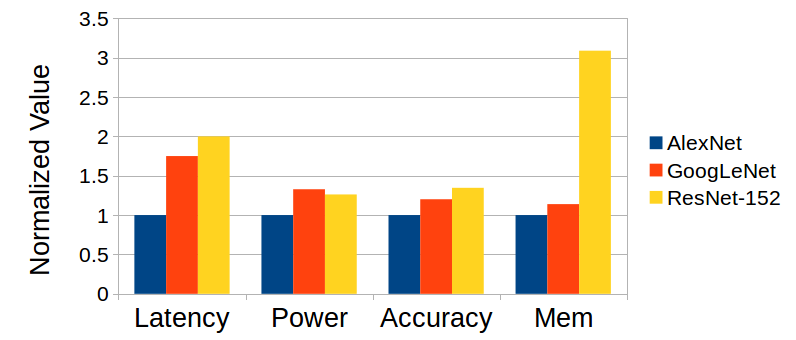
\includegraphics[width=0.5\textwidth]{benchmark_compare.png}
    \caption{Compare the benchmarks in terms of latency, power consumption, memory overhead, and accuracy. The values are normalized to AlexNet. We fix the voltage/frequency pair to the highest one.}\label{fig:3}
\end{figure}